\chapter{Methods}
The aim of drug discovery is to find new chemical entities with desirable pharmacological properties. This is an inherently difficult task due to the vast size and complexity of the chemical search space. The range of drug-like molecules has been estimated to be between 10\textsuperscript{23} and 10\textsuperscript{60} \cite{polishchuk2013estimation}. Meanwhile, the chemical space is discrete, making the search difficult to perform \cite{kirkpatrick2004chemical}. As a result, drug development is a lengthy and costly process, with the average clinical development time for one drug reaching more than nine years and the estimated median development cost 1.1 billion USD \cite{wouters2020estimated}.

\section{Data set}
ZINC is a database of over 100 million small organic molecules \cite{irwin2005zinc}. It is organized into subsets based on the properties of the compounds, including molecular weight and drug-likeliness, enabling the search for compounds with desired characteristics. ZINC is commonly used in computer-aided drug design to identify compounds for medicinal chemistry issues and in other research areas, such as virtual screening and chemical informatics. As such, the database is beneficial for professionals in drug discovery and development as it provides a diverse collection of commercially available compounds for a variety of purposes.

This study randomly sampled 20,000 molecules from 10,071,918 molecules with 18 or less elements (nodes) obtained from the ZINC database. We intentionally seeded the random sampler to allow for future studies. We remedied the deficiencies due to scalability issues by expanding the ZINC data set to include samples with longer sequences. While ZINC molecules comprise 12 types of atoms (B, C, N, O, F, Si, P, S, Cl, Br, Sn, and I), the molecules in our data set only comprise 8 types of atoms (C, N, O, F, Si, S, Cl, Br). We note that this may result in generating molecules without B, P, Sn, and I elements since the VAE models aim to generate molecules that resemble the data set. The sampled molecules have four types of bonds (single, double, triple, and aromatic).

Fig. 2 shows the histograms of the molecular properties in the data set used in this study, with the mean of ClogP $= 0.929$ and CMR $=63.063$.
\begin{figure}[htbp]
    \centerline{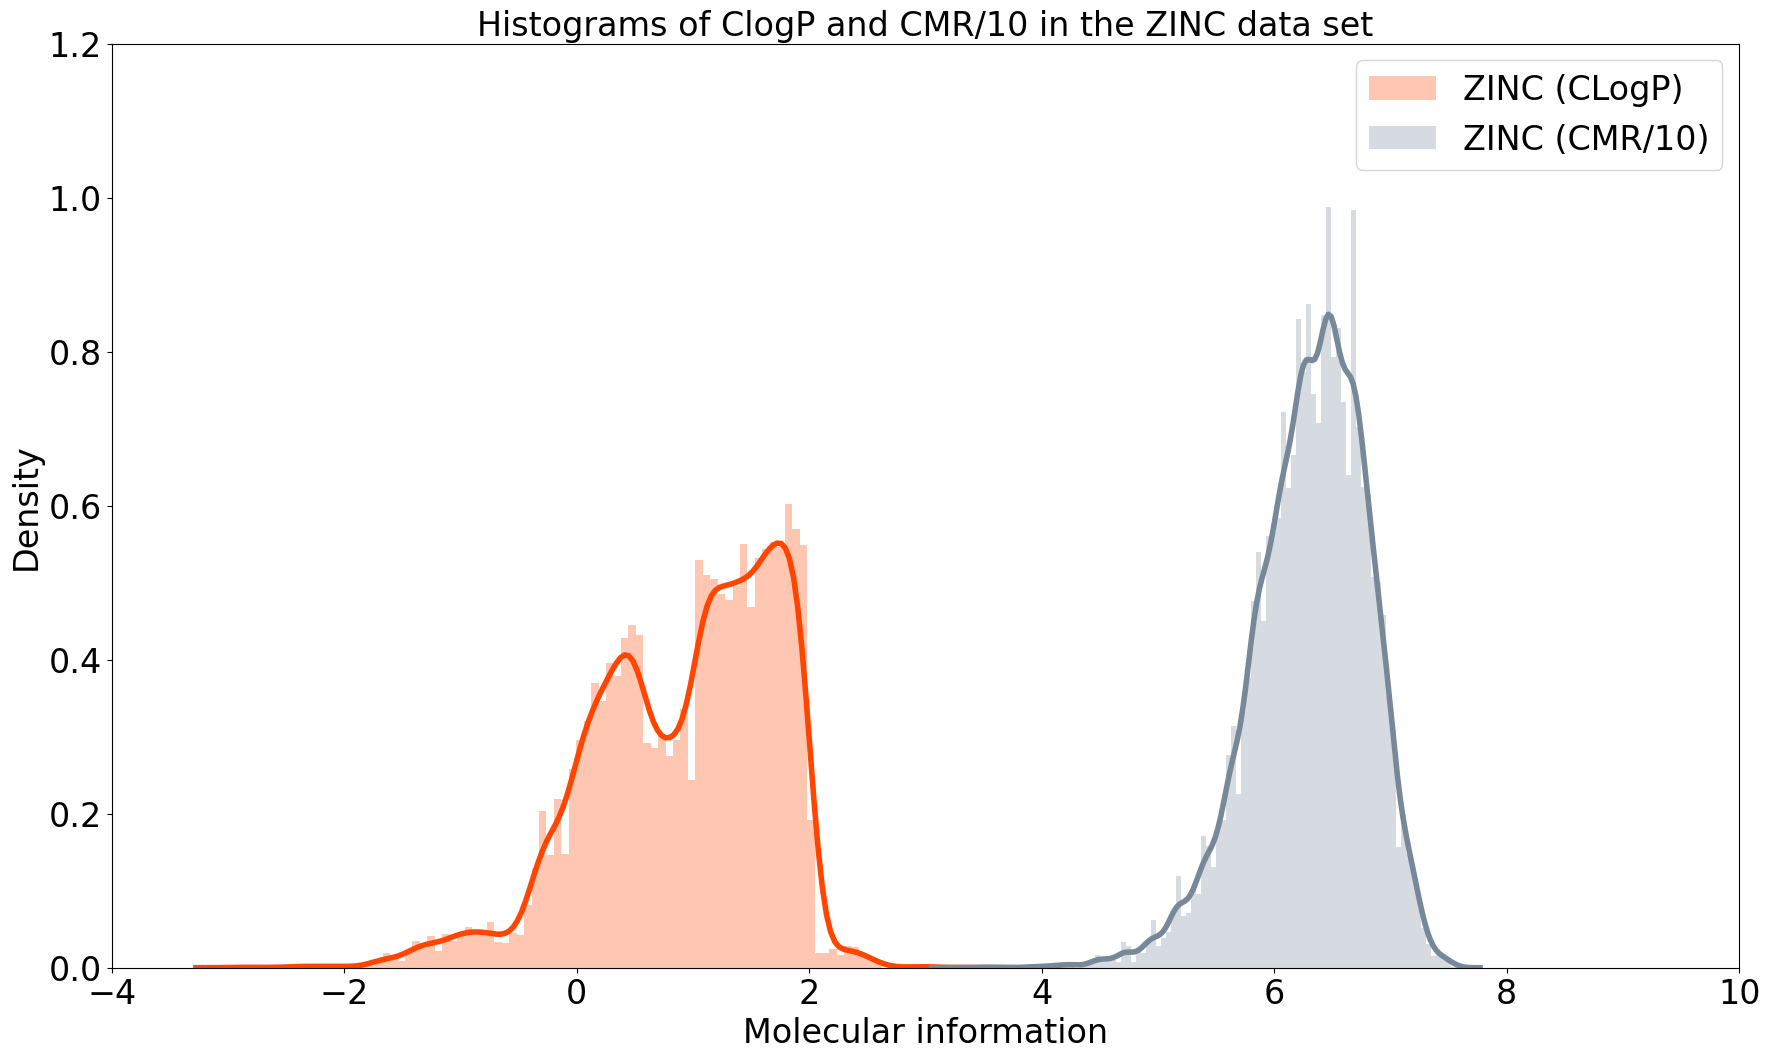
\includegraphics[width=0.7\textwidth]{fig2.png}}
    \caption{Histograms of ClogP and CMR of the data set.}
    \label{fig}
\end{figure}

\subsection{Preprocessing}

\begin{figure*}
    \centering
    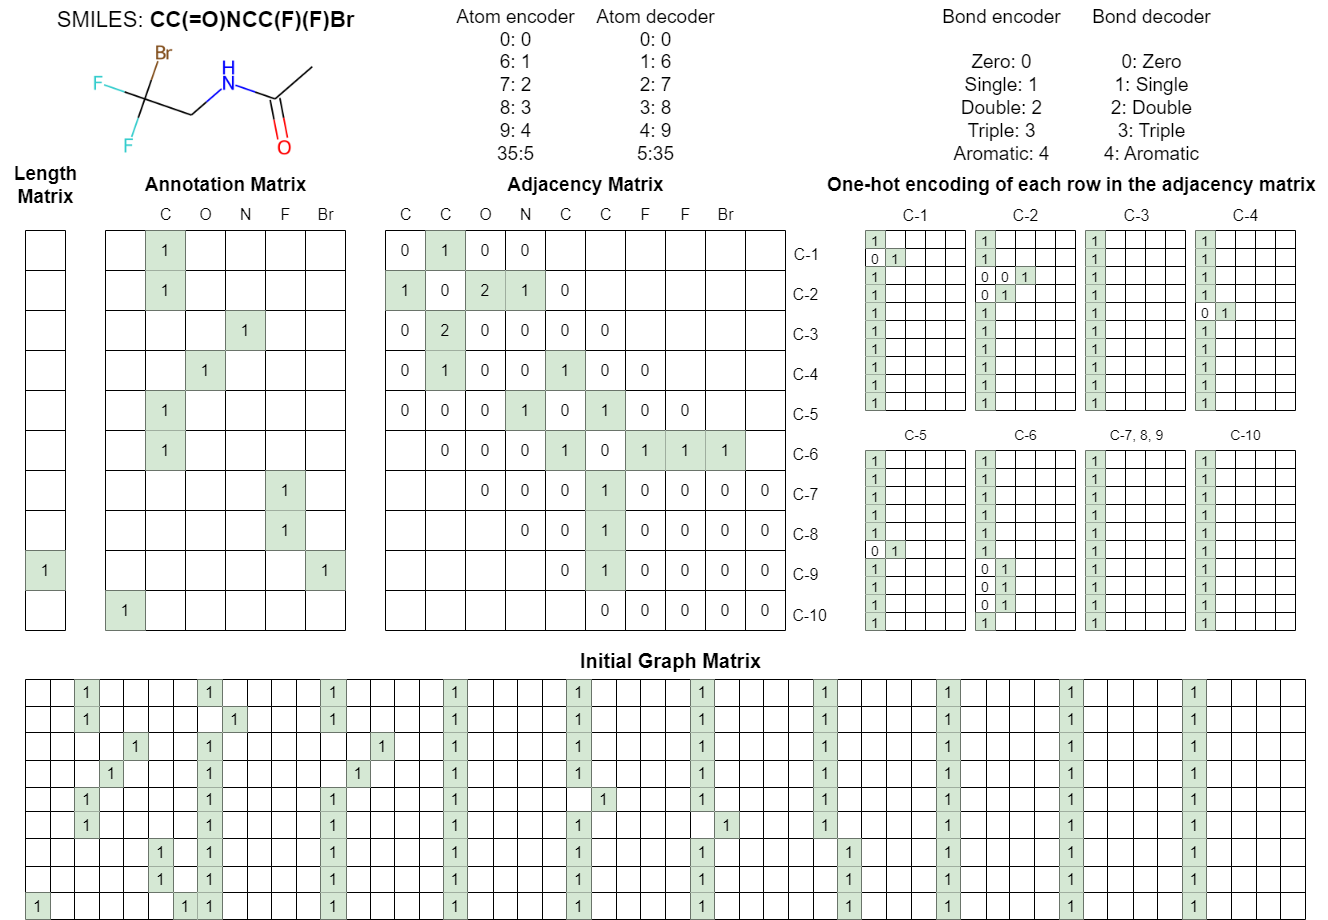
\includegraphics[width=1\textwidth]{fig3.png}
    \caption{Construction of the initial graph matrix for CC(=O)NCC(F)(F)Br. The length matrix encodes the length of the molecule. Here, we use 10 to demonstrate padding in the construction. The annotation matrix encodes each atom and the adjacency matrix describes the bond information \cite{lee2022mgcvae}. To reduce the computational intensity, we consider the upper right triangle of the adjacency matrix (symmetry) to construct the one-hot encoding of each row in the adjacency matrix.}
    \label{fig:img1}
\end{figure*}

To generate molecular graphs, we used RDKit to convert SMILES into molecules through an iterative process \cite{landrum2013rdkit}. Subsequently, we adopted the graph input representation based on the encoding process from \cite{lee2022mgcvae}. The structure of each molecule is represented by an initial graph matrix, which comprises an annotation matrix ($N\times M$) and an adjacency matrix $A$ ($N\times N$), where $N$ denotes the number of atoms and $M$ denotes the number of types of atoms. Fig. 3 shows the construction of the molecule $M1$, CC(=O)NCC(F)(F)Br. To demonstrate simply, we let $N = 10$ be the maximum length of the molecule instead of $N = 18$ in our experiments. Since the length of molecule $M1 = 9$, the length matrix is shaded at the ninth index. In the annotation matrix, each row represents a one-hot encoded atom. The adjacency matrix $A$ represents how each atom is bonded. The symmetric property of the adjacency matrix can be leveraged to reduce computation intensity. Hence, we consider only the upper triangle of the adjacency matrix. The rows of the adjacency matrix denote the type of bonds, denoted from $C\-1$ to $C\-10$. We note that row $i$ and column $j$ for $A(10,j)$ and $A(i,10)$ are padding to the adjacency matrix to ensure that every initial graph matrix of each molecule satisfies the same matrix dimensions. Finally, the length matrix, annotation matrix, and one-hot encoding of each row in the adjacency matrix are concatenated horizontally.  

This method of molecular representation allows the initial graph matrix to be constructed in a unique way. Moreover, the graph matrix of the generated molecule can be reconstructed and converted into SMILES \cite{lee2022mgcvae}. The sampled data set was loaded into a data loader and divided into training and test sets at a ratio of 8:2. 

\subsection{Multi-objective property optimization}
In this study, we aim to generate molecules with optimized ClogP and CMR values. These values are introduced into the latent space of the VAE by using a pairwise condition vector. \cite{ghose1999knowledge} suggested that drug-like molecules have logP $\in [-0.4, 5.6]$ or MR $\in [40, 130]$. We use Crippen's method to predict the molecular properties of logP and MR \cite{wildman1999prediction}. We posit that this method is appropriate for our study because the graph generation process is atom-based as shown in Fig. 3. To that end, we discretize and define the targeted properties with the following values:

\begin{equation}
    \begin{aligned}
    & C1 = ClogP = \{0, 1, 2, 3, 4 \}\\
    & C2 = CMR  =\{20, 30, 40, 50, 60, 70\} \label{eq}
    \end{aligned}
\end{equation}
where $C2 = \{20, 30\}$ is $\notin$ the proposed MR range of the Ghose filter. This is intentionally included in (6) for experimentation and evaluation purposes of the conditional vector. Since (6) is one-hot encoded, we scale C2 by $0.1$.

\subsection{Model}
 We propose the $\beta$-conditional variational autoencoder ($\beta$-CVAE) or conditional $\beta$VAE in this study. The $\beta$-CVAE is an extension of the aforementioned VAEs. We rewrite (5) to define the objective function of $\beta$-CVAE as follows:
\begin{equation}
\begin{split}
\mathbb{E}_{q_\phi(z|x,c)}[log p_\theta(x|z),c] - \beta D_{KL}[q_\phi(z|x,c)\parallel p(z|c)],\label{eq}
\end{split}
\end{equation}
where $\beta$ is the hyperparameter to introduce disentanglement. We set an $\beta = 2$ as an arbitrary value in this study. Fig. 4 shows the model architecture.

\begin{figure}[htbp]
    \centerline{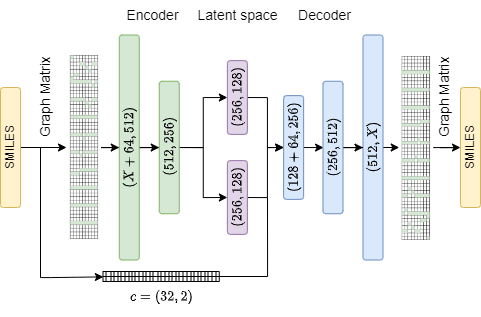
\includegraphics[width=0.7\textwidth]{fig4.png}}
    \caption{$\beta$-CVAE Model Architecture}
    \label{fig}
\end{figure}

\subsection{Network training}
All networks described in this paper were implemented using PyTorch. All training was performed on an NVIDIA GeForce RTX2060 GPU, with 16GB of memory.

Adam optimizer was used during the training of the models and various schedulers were tested to change the learning rate. Subsequently, we used a modified gradient-based optimization algorithm proposed by \cite{DBLP:journals/corr/abs-1909-13371}. The authors modified the backpropagation algorithm for the computation of "hypergradients" to optimize the hyperparameters, such as step size and momentum coefficients. Previously, most DL practitioners have to experimentally set these hyperparameters, which could be a tedious and time-consuming process. This new gradient optimizer, \textit{gdtuo}, permits the optimizer's hyperparameters to be optimized alongside the model parameters during training, rather than having to be manually chosen ahead of time. In this regard, this method can save time and effort by automating the optimization of hyperparameters. Table 1 provides the hyperparameters used to train the $\beta$-CVAE model. We applied the same hyperparameters for the training of $\beta$-VAE, CVAE, and VAE models. Fig. 5 shows our training and test loss curve for 1000 epochs, which suggests overfitting when using  Adam (\textit{gdtuo}) as the optimizer.

\begin{figure}[htbp]
    \centerline{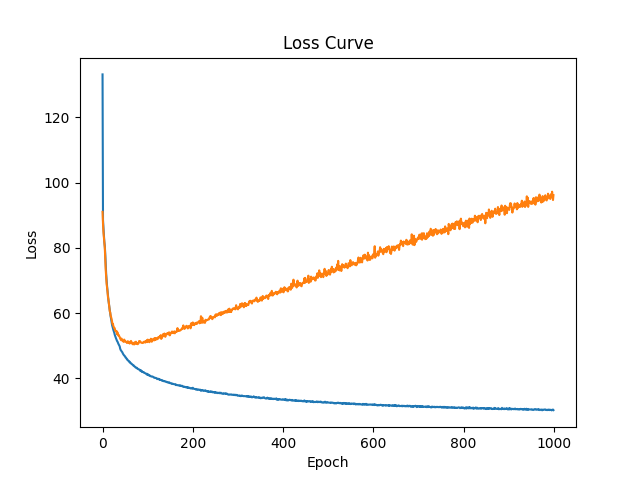
\includegraphics[width=0.45\textwidth]{overfitting.png}}
    \caption{$\beta$-CVAE training-test loss curve using \textit{gdtuo} optimizer}
    \label{fig}
\end{figure}

\begin{table}[htbp]
\caption{Network Training}
\centering
        \begin{tabular}{ll}
        \hline
        Hyperparameter & Value \\ \hline
        Optimizer type & Adam and Adam \textit{gdtuo} \\
        Learning rate & 0.005 (Adam) \\
        Number of epochs & 1000 (Adam) \\
        Batch size & 100 (Adam) \\
        $\beta$ & 4 (Adam) \\ \hline
        \end{tabular}
        \label{tab1}
\end{table}

\subsection{Evaluation methods}
The model performance was evaluated by generating molecules with the target properties defined in (6). We  compared the number of generated molecules that satisfies these properties. We first compare the generated results of every model with the data set. The percentage scores of ClogP and CMR refer to the percentage of molecules within the Ghose filter, where ClogP $\in [-0.4, 5.6]$ and CMR $\in [40, 130]$. We conduct single-property evaluations before evaluating the molecular properties simultaneously. Secondly, we compare the conditional models with the non-conditional models based on the target properties. We defined the molecular properties to be within the range of the conditional value in (6) if $C1 \pm 0.5$ and $C2 \pm 5$. This was done to determine the performance of each model and to compare the results more clearly.

As a second metric to further access the model performance, the following metrics are considered: validity (the proportion of valid molecules among all generated molecules), novelty (the proportion of valid molecules that are not present in the training data set), and uniqueness (the proportion of unique, valid molecules, which reflects the diversity of the generated samples). 
